\documentclass[12pt]{report}
\usepackage[spanish]{babel}
\usepackage[utf8]{inputenc}
\usepackage{graphicx}
\usepackage{verbatim}
\usepackage{listings}
\usepackage{float}
\renewcommand*\thesection{\arabic{section}}

\begin{document}
	
	\begin{center}
		\textbf{Análisis de Algoritmos, Sem: 2018-1, 3CV1, Práctica 8, 11-2017}
		\newline
	\end{center}
	
	\begin{center}
		\begin{picture}(0,0) \put(-125,-55){
			\includegraphics[width=2.7cm]{../../IPNlogo.jpg}} 
		\end{picture}
		\LARGE Escuela Superior de Cómputo.\\
		Instituto Politécnico Nacional, México.\\
		\begin{picture}(0,0) \put(160,10){
			\includegraphics[width=2.7cm]{../../logoescom.png}} 
		\end{picture}
	\end{center}
	
	\begin{center}
		\Large Práctica 8: Subsecuencia común más larga.\\
	\end{center}
	
	\begin{center}
		\textbf{Blancas Pérez Bryan Israel}\\
		orionmunecaycanica@gmail.com\\
	\end{center}
	
	
	\textbf{\large Resumen: }Implementar el algoritmo de la subsecuencia común más larga, con el enfoque de programación dinámica, para hallar que tan similares son dos archivos analizados. \newline\\
	\textbf{\large Palabras Clave: } Subsecuencia común más larga, Programación dinámica, Similitud entre cadenas, Complejidad Computacional.\\
	


	\section{Introducción}
	La programación dinámica, es un método para reducir el tiempo de ejecución de un algoritmo.[1]. Este método, proporciona un procedimiento sistemático para encontrar la combinación de decisiones que maximice la efectividad total, descomponiendo el problema en etapas, y al final enlazando cada etapa a través de recursividad.[2] \newline
	En está práctica, se aplicará este método de programación para resolver el problema de encontrar la subsecuencia común más larga entre dos cadenas de texto, en un tiempo razonable a comparación del algoritmo por fuerza bruta.\newpage
	
	
	\section{Conceptos Básicos}
	\textbf{Subsecuencia Común Más Larga}\\
		
El problema de la Subsecuencia Común Más Larga, (Longest Common Subsequence, LCS por sus siglas en inglés) trata de encontrar una subsecuencia más larga que es común en un conjunto de secuencias. El problema de LCS es uno de los problemas clásicos de las ciencias computacionales y es la base de programas que comparan datos, y tiene varios usos, como en la bioinformática. [3]\\
Cabe destacar, que para un número grande se secuencias a comparar, este problema se considera NP-hard. En esta práctica, solo obtendremos el LCS de dos secuencias;  el algoritmo implementado aquí, está hecho bajo el paradigma de programación dinámica, con un tiempo computacional $O(mn)$, donde m y n son las longitudes de las dos secuencias.\\

	
	Ejemplo de una subsecuencia común:\\
	
	Sea $A:<XMJYAUZ>$ y $B:<MZJAWXU>$, entonces el LCS (llamado $C$), sería $C:<MJAU>$.\\
	
	Con este ejemplo, se aprecia, que no importa que las letras estén juntas, la única condición es que deben de estar en el mismo orden (secuencia).\\
	
	Usando la programación dinámica para encontrar el LCS, el algoritmo construye una matriz L[0..m, 0..n] donde L(i, j) representa el LCS para x1 . . . i y y1 . . . j. Cada valor en la matriz se calcula basándose en los valores de las posiciones vecinas anteriores.[4]
		\begin{figure}[H]
			
\includegraphics[height=3cm,width=9cm]{imagenes/1.png}
			\centering
			\caption{Ecuación para el algoritmo.}
			\centering
		\end{figure}
		\newpage
		
	La matriz generada para el ejemplo de la página anterior se muestra en la figura 2, en donde está remarcado de color amarillo el camino de la LCS, y con números remarcados, el carácter correspondiente. \\
		\begin{figure}[H]
			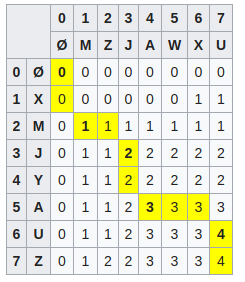
\includegraphics[height=9cm,width=9cm]{imagenes/2.png}
			\centering
			\caption{Ecuación para el algoritmo.}
			\centering
		\end{figure}
	\newpage

	\section{Experimentación y Resultados}	
	\textbf{Ejercicio 1.}\\
Implementar un programa que como entrada tenga dos archivos en modo de texto y
como salida muestre en porcentaje que tan parecidos o similares son lo archivos. Para ello:\\
i) Omita espacios, es decir, los espacios no se consideran.\\
ii) Reporte 5 parejas de ejemplos donde muestre el porcentaje de similitud.\\
	
	
	Pseudocódigo del algoritmo:
	\lstset{language=C, breaklines=true, basicstyle=\footnotesize}
	\lstset{numbers=left, numberstyle=\tiny, stepnumber=1, numbersep=10pt}
	\begin{lstlisting}
LCS(X[1..m], Y[1..n])
  C = array(0..m, 0..n)
  for i = 0 to m do
    C[i,0] = 0
  for j = 0 to n do
    C[0,j] = 0
  for i = 1 to m do
    for j = 1 to n do
      if X[i] == Y[j]
        C[i,j] = C[i-1,j-1] + 1
      else
        C[i,j] = max(C[i,j-1], C[i-1,j])
return C[m,n]  

findLCS(C[0..m,0..n], X[1..m], Y[1..n], i, j)
  if i = 0 or j = 0
    return ""
  else if  X[i] = Y[j]
    return findLCS(C, X, Y, i-1, j-1) + X[i]
  else
    if C[i,j-1] > C[i-1,j]
      return findLCS(C, X, Y, i, j-1)
    else
      return findLCS(C, X, Y, i-1, j)
	\end{lstlisting}
	
		
La función LCS, crea la matriz solución, mientras que la función findLCS, encuentra la subsecuencia común más larga.\newpage
	
	\textbf{Pareja 1.}\\
	Input.\\
	A: (100 de semejanza).\\
	B: (100 de semejanza).\\	
	Output.\\	
	\begin{figure}[H]
		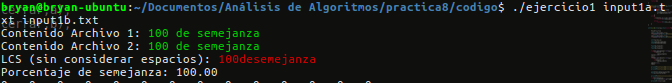
\includegraphics[height=2.2cm,width=15cm]{imagenes/3.png}
		\centering
		\caption{Pareja 1.}
		\centering
	\end{figure}
	Como las dos cadenas son exactamente iguales, el porcentaje de semejanza es 100.\\	
	Ejemplo de matriz solución generada (por estética del reporte, en las siguientes ejecuciones no pondré la matriz):
	\begin{figure}[H]
		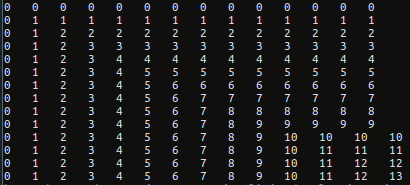
\includegraphics[height=7cm]{imagenes/3-1.png}
		\centering
		\caption{Matriz solución-Pareja 1.}
		\centering
	\end{figure}
	  \newpage
	
	\textbf{Pareja 2.}\\
	Input.\\
	A: (veamos que tan semejantes con este archivo 2a).\\
	B: (con este otro archivo 2b).\\	
	Output.\\	
	\begin{figure}[H]
		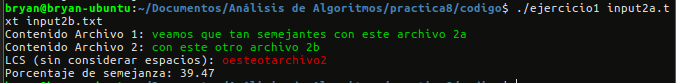
\includegraphics[height=2.2cm,width=15cm]{imagenes/4.png}
		\centering
		\caption{Pareja 2.}
		\centering
	\end{figure}

	\textbf{Pareja 3.}\\
	Input.\\
	A: (There's a lady who's sure All that glitters is gold And she's buying a stairway to heaven When she gets there she knows If the stores are all closed With a word she can get what she came for Oh oh oh oh and she's buying a stairway to heaven).\\
	B: (Nobody gonna take my car I'm gonna race it to the ground Nobody gonna beat my car It's gonna break the speed of sound Oooh it's a killing machine It's got everything Like a driving power big fat tires And everything).\\	
	Output.\\	
	\begin{figure}[H]
		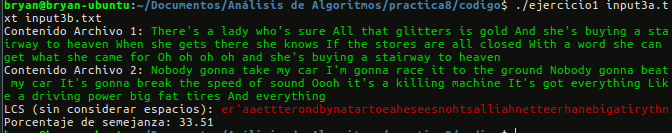
\includegraphics[height=3cm,width=15cm]{imagenes/5.png}
		\centering
		\caption{Pareja 3.}
		\centering
	\end{figure}
	
	\newpage
	
	\textbf{Pareja 4.}\\
	Input.\\
	A: (El Longest common subsequence problem (Problema de subsecuencia común más larga) también conocido como LCS problem, se trata de encontrar una subsecuencia más larga que es común en un conjunto de secuencias (Aunque en la mayor parte solamente se toman dos secuencias).).\\
	B: (La subsecuencia es cualquier subconjunto de elementos que mantienen el orden, entonces el problema de encontrar la subsecuencia común mas larga se define como : Dadas 2 cadenas , sean X e Y, encontrar la longitud de la cadena mas larga Z, tal que los caracteres de Z aparezcan en en ese mismo orden dentro de las cadenas X e Y.).\\	
	Output.\\	
	\begin{figure}[H]
		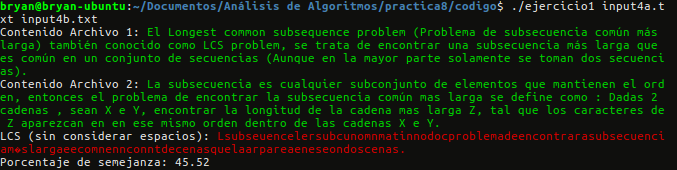
\includegraphics[height=3cm,width=15cm]{imagenes/6.png}
		\centering
		\caption{Pareja 4.}
		\centering
	\end{figure}
	
	\textbf{Pareja 5.}\\
	Input.\\
	A: (bryan israel blancas pérez).\\
	B: (antonio issac blancas pérez).\\	
	Output.\\	
	\begin{figure}[H]
		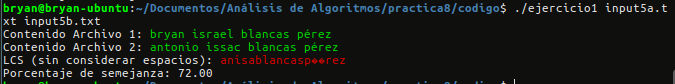
\includegraphics[height=3cm,width=15cm]{imagenes/7.png}
		\centering
		\caption{Pareja 5.}
		\centering
	\end{figure}

\newpage		
\section{Conclusiones}
Esta práctica me gustó mucho, porque programar el algoritmo tiene cierto grado de complejidad, sobretodo en fijarse bien en los índices de los arreglos. Además, este ejemplo es muy bueno para ejemplificar el uso de la programación dinámica, pasando de un tiempo computacional muy grande para el algoritmo de fuerza bruta, a un tiempo razonable aplicando ésta técnica.\\
Pienso que esta práctica es buena para mejorar las técnicas de programación y para la lógica detrás de encontrar un algoritmo eficiente para la resolución de un problema.
\newpage 

\section{Bibliografía}

[1] https://es.wikipedia.org/wiki/Programación\_dinámica.\\

[2] http://www.ingenieria.unam.mx/sistemas/PDF/Avisos/Seminarios/\\SeminarioV/Sesion6\_IdaliaFlores\_20abr15.pdf\\

[3] https://es.wikipedia.org/wiki/Problema\_de\_Subsecuencia\_Comú\_mas\_Larga\\

[4] http://www.bdigital.unal.edu.co/2754/1/299716.2010.pdf
	
		
\end{document}